\section{实验结果}
\subsection{LoRA 实现与功能验证}
手工实现在Qwen 基础模型上完成了注入、参数统计、前向计算和合并。实际替换 \ReplacedCount{} 个线性层，新增可训练参数为 \TrainableCount{}，含适配器的总参数为 \TotalCount{}，比例为 \TrainableRatio{}。这说明实现能够以较小的可训练参数集合工作，但该比例不代表实测显存节省。

九项测试覆盖初始等价、共享原权重、非零修正、合并等价及幂等、模块替换、非法配置、数据划分和真实奖励 HTTP 接口。其中小层测试实际执行了优化器更新，确认冻结参数不变。原 \code{main()} 本身没有优化器步骤，故其打印成功不能单独证明语言模型微调效果。完整输出与实现说明见附录~\ref{app:implementation-zh}。

\subsection{完整参数优化实验与同条件验证}
2026 年 11 月 8 日的 A10 BF16 实验完成 512 道训练题、\PPORolloutSteps{} 批采样，训练进程以退出码 0 结束；进度条显示训练循环约 12 分 02 秒，不含模型下载、安装、训练前后评估。独立的 16 题保存与 Actor 重载检查先通过，完整运行随后重新从原始基座开始。

Actor 的 \PPONonzeroBTensors{}/\PPOBTensors{} 个 LoRA B 张量、Critic 的 \PPOCriticNonzeroBTensors{}/\PPOCriticBTensors{} 个 B 张量非零；下载的全部适配器值和记录的标量均为有限数。与只看“开始运行”的日志相比，这些检查直接支持参数已更新并保存。

\par\noindent\begin{minipage}{\linewidth}
\tablecaption{tab:paired-zh}{同一组 128 道开发验证题的配对结果。}
\begin{tabularx}{\linewidth}{@{}Y P{38mm}P{38mm}@{}}
\toprule
\tablehead \key{指标} & \key{训练前} & \key{训练后}\\
\midrule
首行整数答案正确题数 & \PPOBaselineCorrect{}/\PPOValidationN & \PPOTrainedCorrect{}/\PPOValidationN\\
正确率 & \PPOBaselineAccuracy & \PPOTrainedAccuracy\\
相对基线的绝对变化 & --- & \PPODelta{} 个百分点\\
\bottomrule
\end{tabularx}
\end{minipage}\par


逐题复核发现：117 题前后均正确，5 题由错变对，6 题前后均错，没有由对变错的题。净增加 5 道正确答案与总体差值一致。两次评估使用相同 BF16 精度、贪心解码、生成长度和评分规则；图~\ref{fig:paired-zh} 保留每一道题，而不只展示两个汇总百分比。

\begin{minipage}{\linewidth}
\par\noindent\begin{minipage}{\linewidth}
\begin{center}
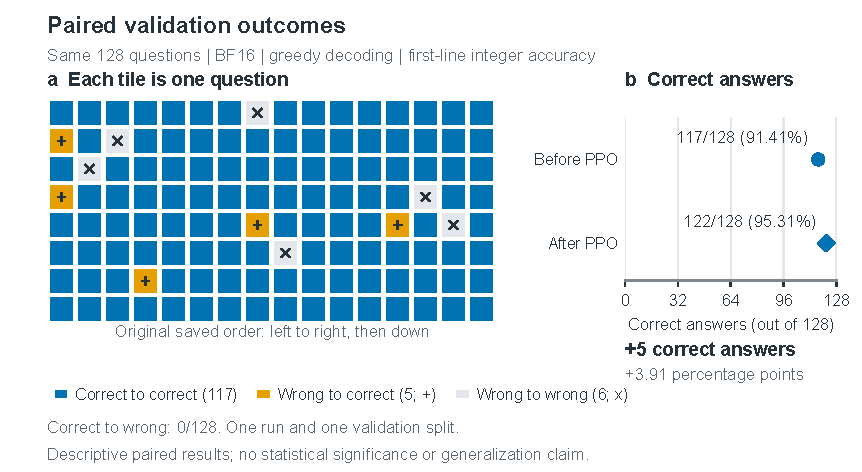
\includegraphics[width=146mm]{../../figures/paired_validation_outcomes.pdf}
\end{center}
\figcaption{fig:paired-zh}{保存题序中的 128 道题逐题配对。左图每格一题：117 题均正确、5 题由错变对、6 题均错误；右图给出正确数和正确率。每个状态均由原始回答重新评分，没有新增题目、重排以增强效果或添加统计显著性结论。}
\end{minipage}\par

\end{minipage}

\smallheading{保存与重载的实际范围}
Actor 已与基础模型一起在 GPU 上重新加载，通过有限值前向计算和生成检查。Critic 适配器通过哈希、有限值及非零更新检查，\key{没有独立重载 Critic}。保存的内容是 LoRA 适配器，不含基础模型权重，也不是可以完整恢复 PPO 优化器状态的检查点。原始回答、配置、标量指标和适配器保存在 \path{policy_adaptation/results/}。

\begin{minipage}{\linewidth}
\par\noindent\begin{minipage}{\linewidth}
\begin{center}
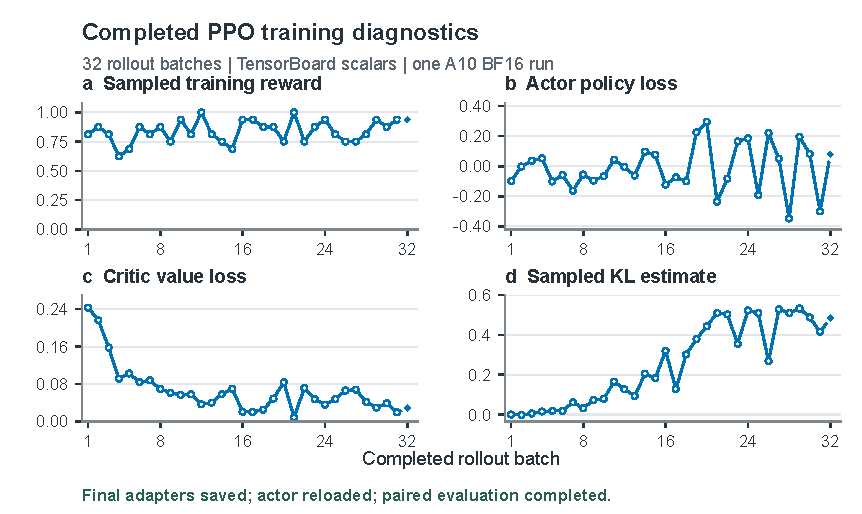
\includegraphics[width=146mm]{../../figures/ppo_training_success.pdf}
\end{center}
\figcaption{fig:ppo-curves-zh}{成功运行的四项训练诊断，每条曲线包含全部 32 个采样批次，每批 16 题。来自原始事件的数值未平滑，也未给单次运行添加置信区间。训练随机采样回答，温度为 1、top-$p$ 为 1；开发验证则使用贪心解码。}
\end{minipage}\par

\end{minipage}

平均任务奖励会随题目和采样回答波动，不能把首批与末批奖励之差解释成同条件正确率变化。Actor 策略损失可以为负，正负号不等于回答优劣；Critic 损失反映价值预测误差。记录的 KL 是采样估计，可能略小于零；理论 KL 散度本身仍非负。最后一批平均任务奖励为 0.9375，不能直接替代训练后验证正确率 0.953125。

\subsection{程序搜索的实际在线进展}
在线工程保存了 7 个方案记录：5 个完成有效评估，1 个因 Python 语法错误未能实现，另 1 个尚未评估。图表只统计实际完成且合法的结果，失败或缺失不会被填成零分。

\par\noindent\begin{minipage}{\linewidth}
\tablecaption{tab:online-scores-zh}{五次有效在线评估。时间均为 2026 年 10 月 31 日 UTC+08:00；第 0 代表示初始化。}
\begin{tabularx}{\linewidth}{@{}P{28mm}P{12mm}P{12mm}P{29mm}Y@{}}
\toprule
\tablehead \key{候选编号} & \key{代数} & \key{岛} & \key{分数} & \key{记录时间}\\
\midrule
\code{fe0aad416d4f} & 0 & 0 & 2.473873492 & 12:46:55\\
\code{4705b8e92e1b} & 0 & 1 & \key{2.620013807} & 13:08:21\\
\code{d3fb7a9f0bab} & 0 & 1 & 2.464972339 & 13:10:19\\
\code{34836c89e4f0} & 1 & 1 & 2.616027976 & 13:18:13\\
\code{a15ea29f0ceb} & 1 & 0 & 2.514353475 & 13:18:47\\
\bottomrule
\end{tabularx}
\end{minipage}\par


\begin{minipage}{\linewidth}
\par\noindent\begin{minipage}{\linewidth}
\begin{center}
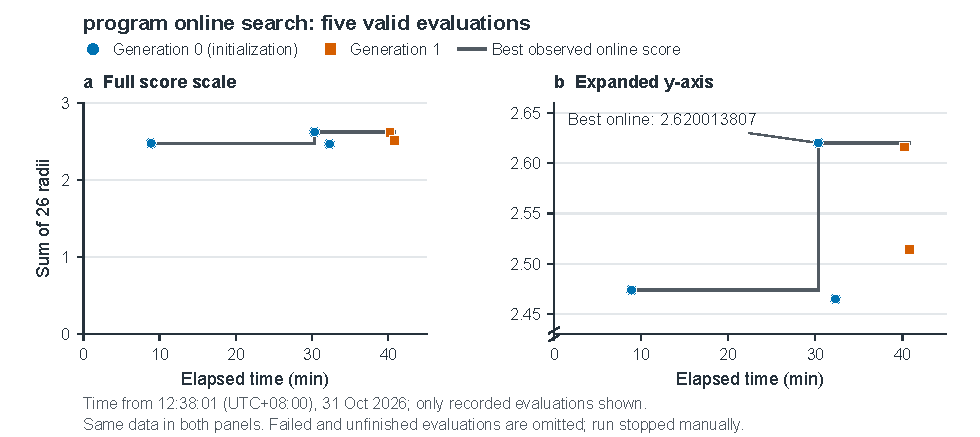
\includegraphics[width=166mm]{../../program_search/figures/online_progress.pdf}
\end{center}
\figcaption{fig:search-progress-zh}{同一组五次有效在线分数。左侧采用完整纵轴，右侧明确展示放大尺度；圆点为初始化，方点为第 1 代，阶梯线为累计最佳。没有推断第一条记录之前或最后一条之后的结果。}
\end{minipage}\par

\end{minipage}

累计最佳只对已经验证的集合定义：
\[
S_t^\star=\max_{a\in\mathcal V_t}S(a),\qquad \mathcal V_t\ne\varnothing.
\]
第一个分数为 2.473873492，之后一个初始候选达到完整精度的 2.62001380699489。第 1 代的坐标搜索子程序把自己的父程序从 2.473873492 提高到 2.514353475，但这一代的两个新程序都未超过全局最佳。结果证明流程能够生成、执行和筛选程序，不证明每代必然进步或找到了最优布局。

\subsection{最佳程序的独立复现}
导出的最佳候选 \code{4705b8e92e1b} 尝试 8 种固定初始布局，以 SLSQP 同时调整圆心和半径。圆心固定时，再求解
\[
\max_{\boldsymbol r}\ \sum_i r_i
\quad\text{满足}\quad
0\le r_i\le b_i,\quad r_i+r_j\le d_{ij},
\]
其中 $b_i=\min(x_i,y_i,1-x_i,1-y_i)$，$d_{ij}=\|\boldsymbol c_i-\boldsymbol c_j\|_2$。这是给定圆心下的线性规划；随后保守缩小半径以减轻浮点约束误差，不能由此证明圆心布局全局最优。

\begin{minipage}{\linewidth}
\begin{minipage}[c]{0.47\linewidth}
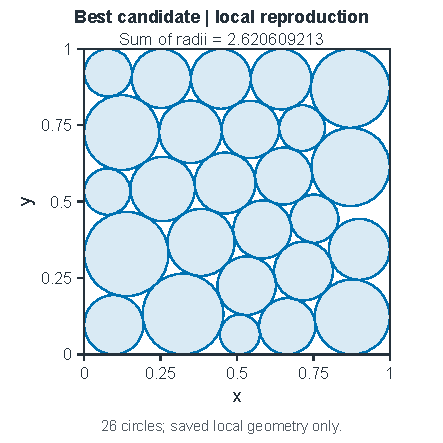
\includegraphics[width=75mm]{../../program_search/figures/online_best_reproduced.pdf}
\end{minipage}\hfill
\begin{minipage}[c]{0.49\linewidth}
\raggedright
未改动的导出程序在 Python 3.14.2、NumPy 2.4.4、SciPy 1.17.1 下约 4.76 秒完成本地复算。原几何方法接受全部 26 个圆；最小边界和圆间间隙约为 $1.38\times10^{-12}$ 与 $1.02\times10^{-12}$，均为正。

\key{在线记录：}2.62001380699489。\\
\key{本地复现：}2.6206092130170973。
\end{minipage}
\figcaption{fig:packing-zh}{最佳导出程序的本地复现布局。圆心、半径来自保存的几何数据，保持等比例，没有重新猜画位置。这不是服务器的原始坐标，也不是平台截图。}
\end{minipage}

两项分数约差 0.000595406。数值库或运行环境差异是一种可能解释，根因未证实。在线分数继续作为在线搜索结果，本地分数只支持独立复现记录；初始构造程序的本地值 0.959764 也不作为同一次在线实验的基线来计算百分比提升。
